In this section we will test the Argyris basis functions and the transformation
that has been developed. This will be done by implementing a finite element
solution to the Biharmonic equation.

Consider the Biharmonic equation in the unit square $\Omega$
\begin{subequations} \label{eqn:problem}
\begin{align}
	\Delta^2 u &= f \text{ on } \Omega \label{eqn:biharmonic}\\
	u= \frac{\partial u}{\partial n} &= 0 \text{ on } \partial \Omega
	\label{eqn:boundary}
\end{align}
\end{subequations}
\subsection{Finite Element Formulation}
Multiplying the left and right of \eqref{eqn:biharmonic} by $v\in
H^{2}_0(\Omega)$ and integrating over $\Omega$ gives
\begin{equation*}
	\int_{\Omega}\! \Delta^2 u v \,dA = \int_{\Omega}\! fv \,dA.
\end{equation*}
Now using the divergence theorem on the left side gives
\eqref{eqn:boundary}
\begin{align*}
	\int_{\Omega}\! \Delta^2 u v \,dA & = \int_{\Omega}\! \nabla \cdot
		\left( \nabla^3 u v \right) - \nabla^3 u \nabla v \,dA \\
  &= \cancelto{0}{\int_{\Delta\Omega}\! \left(\nabla^3 u \cdot \mathbf{n}\right) v \,dS} -
    \int_{\Omega} \nabla \cdot \left(\Delta u \nabla v\right) - \Delta u \Delta v \,dA \\
  &= \cancelto{0}{\int_{\Delta\Omega}\! \Delta u \frac{dv}{d\mathbf{n}} \,dS} +
    \int_{\Omega} \Delta u \Delta v \,dA \\
  &= \int_{\Omega} \Delta u \Delta v \,dA.
\end{align*}
Therefore, let 
\begin{align*}
	a(u,v) &= \int_{\Omega}\! \Delta u \Delta v \,dA \\
	(F,v) &= \int_{\Omega}\! fv \,dA
\end{align*}
and so the problem can be reformulated to 
\begin{equation}
	\begin{split}
	\text{\emph{Find $u \in H^2_0(\Omega)$ such that}}\quad \\ 
	a(u,v) = (F,v) \quad \forall v \in H^2_0(\Omega).
	\end{split}
\end{equation}
Now let $\mathcal{T}_h$ be the set of non overlapping triangles $K$, and let
$V_h$ be the set of $v_h$ such that $v_h$ is in $\mathbb{P}_5(K)$ and fits the
Argyris criteria in Table ()<++> then $v_h \in H^2(\Omega)$. So,
our problem can be reformulated to
\begin{equation}
	\begin{split}
	\text{\emph{Find $u_h \in H^2_0(\Omega)$ such that}}\quad \\ 
	a(u_h,v_h) = (F,v_h) \quad \forall v_h \in H^2_0(\Omega).
	\end{split}
\end{equation}

\subsection{Boundary Conditions}
Since the Argyris Element is of type Hermite, we must be careful to satisfy the
boundary conditions. That is, we not only need to force $u=0$ on $\partial
\Omega$, but we me must also force $\nicefrac{\partial u}{\partial
\mathbf{n}} = 0$ on $\partial \Omega$. 

For the given domain $\Omega=[0,1]\times[0,1]$, we see that along both the lines
$x=0$ and $x=0$ the condition $u=0$ and $\nicefrac{\partial u}{\partial
\mathbf{n}} = \nicefrac{\partial u}{\partial x}$ implies $\nicefrac{\partial
u}{\partial y} = 0,\; \nicefrac{\partial^2 u}{\partial x \partial y}$ and 
$\nicefrac{\partial^2 u}{\partial y^2}=0$ since $u$ is constant in the $y$
direction on these lines.  Similarly, along the lines $y=0$ and
$y=1$ the conditions $u=0$ and $\nicefrac{\partial u}{\partial \mathbf{n}} =
\nicefrac{\partial u}{\partial y} = 0$ implies $\nicefrac{\partial
u}{\partial x} = 0,\; \nicefrac{\partial^2 u}{\partial x \partial y}$ and
$\nicefrac{\partial^2 u}{\partial x^2}=0$ since $u$ is constant in the $x$
direction on these lines.

To enforce these boundary conditions the corresponding $u^h_i$ will be set to
zero and only the system containing interior nodes will be considered for the
linear system. For non-rectangular domains things are a bit more complicated,
since linear combinations of $\nicefrac{du}{dx}$ and $\nicefrac{du}{dy}$ will
have to be zero. The linear combination will depend on the direction of the
normal vector $\mathbf{n}$ corresponding the side of the domain. This more
complicated Neumann boundary condition has not been implemented as of yet, and
so is not considered in the current numerical study.

\subsection{Global Node Numbering}
Different node orderings in a mesh corresponds to permutations of the stiffness
matrix, and since memory use, and convergence speed of iterative methods may
depend on the ordering used it is important to pick a node number that is most
efficient \cite{Fairag}. The node numbering used and that will be
described was taken from Fairag \emph{et. al.}, since they demonstrated that it
resulted in a stiffness matrix that had the desired properties, i.e. a banded
matrix.

The node ordering consisted of first numbering the vertices of each triangle
with six successive numbers and then numbering the midpoint nodes starting,
first, with the horizontal sides, followed by the vertical and oblique sides. An
illustration of the node number can be found in Figure \ref{fig:NodeNum}.

\begin{figure}[h]
	\begin{center}
    \begin{tikzpicture}[scale=0.4]
\tikzstyle{every node}=[font=\tiny]
      \draw (0,0) node[below left,fill=none]
      {$\begin{array}{l}1,\\2,3\\4,5,6\end{array}$} 
      -- (3,0) node[below,fill=none] {$25$}
      -- (6,0) node[below right,fill=none]
      {$\begin{array}{l}7,\\8,9\\10,11,12\end{array}$} 
      -- (6,3) node[above right,fill=none] {$29$}
      -- (6,6) node[above right,fill=none] 
      {$\begin{array}{l}19,\\20,21\\22,23,24\end{array}$} 
      -- (3,6) node[above,fill=none] {$26$}
      -- (0,6) node[above left,fill=none]
      {$\begin{array}{l}13,\\14,15\\16,17,18\end{array}$} 
      -- (0,3) node[above left,fill=none] {$27$}
      -- cycle;
      \draw (0,0) -- (3,3) node[above left,fill=none] {$28$} -- (6,6);
    \end{tikzpicture}
	\end{center}
  \caption{Global node numbering.}
	\label{fig:NodeNum}
\end{figure}


This node numbering resulted in a banded matrix that can be seen graphically in
Figure \ref{fig:MatrixGraph}.

\begin{figure}[h]
	\begin{center}
    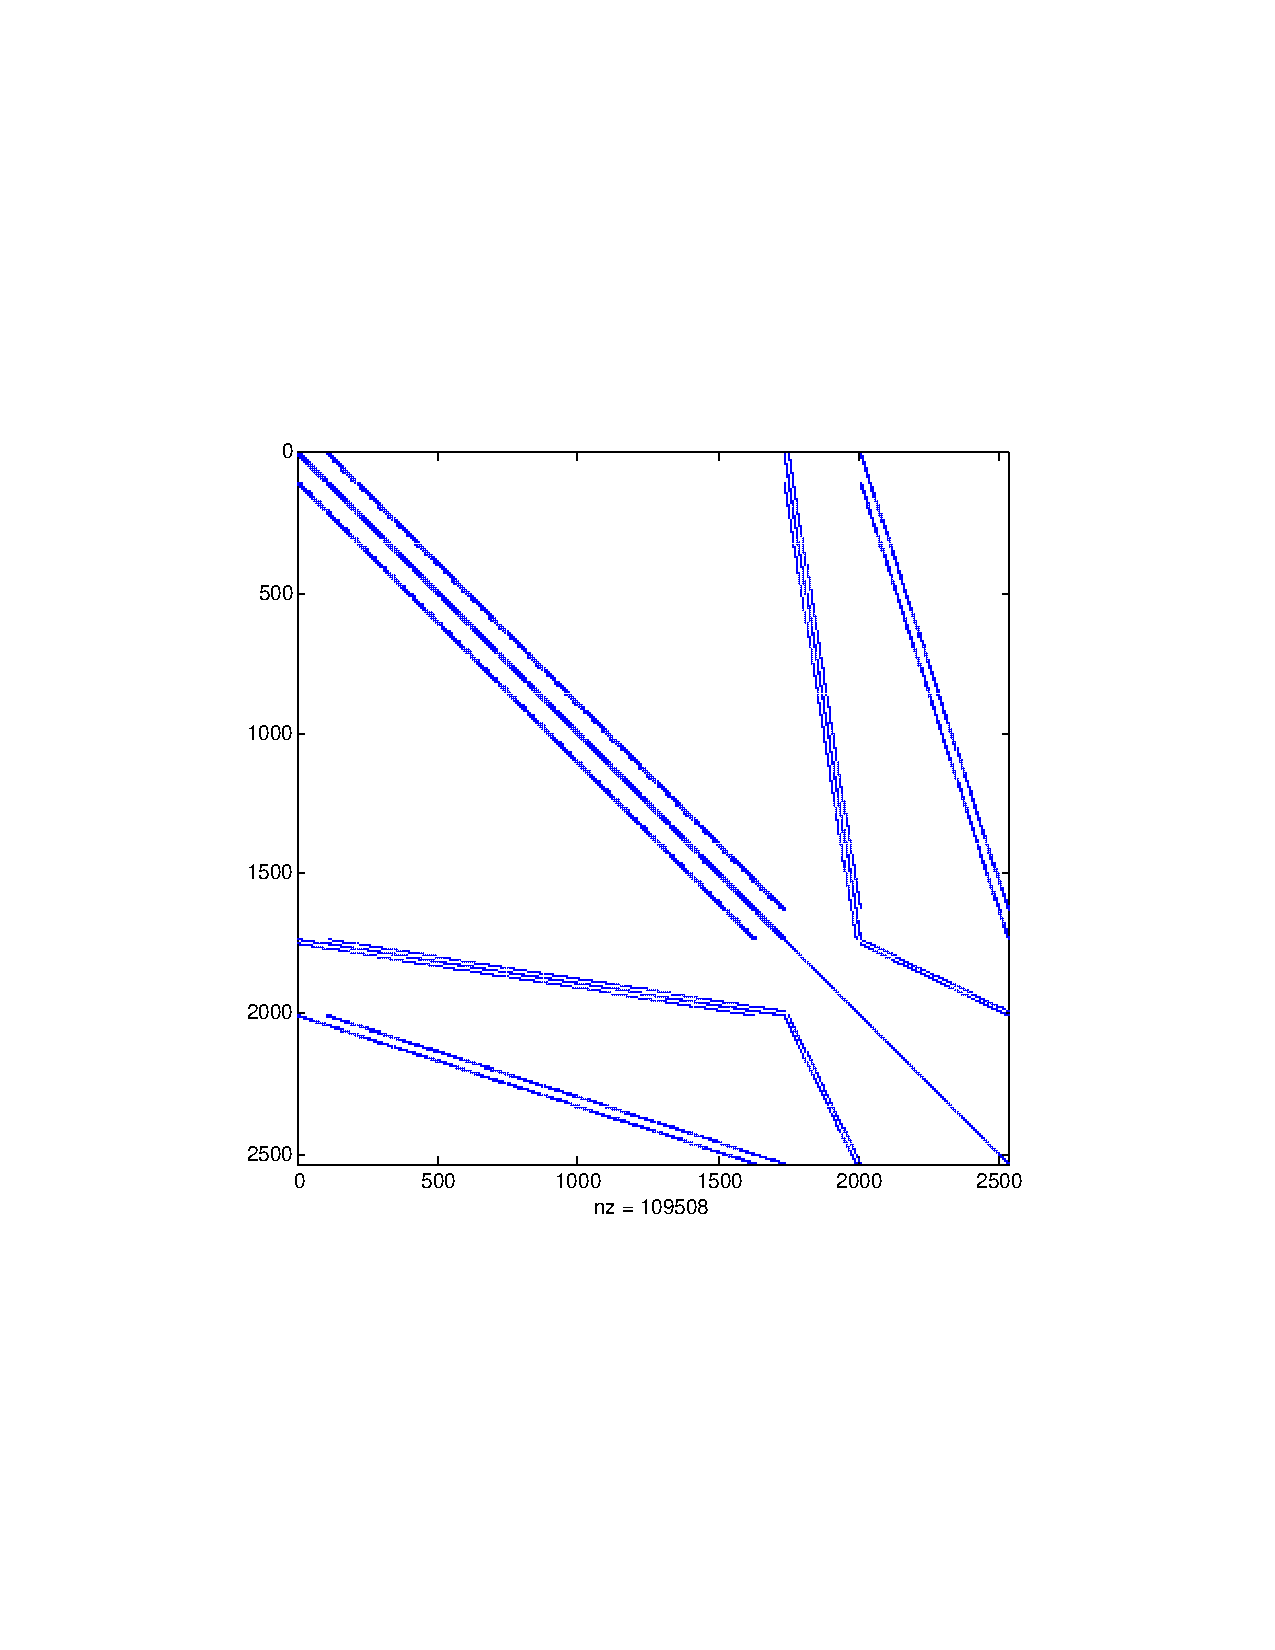
\includegraphics[trim=100 235 100 250, clip, scale=0.5]{Matrix.pdf}
	\end{center}
  \caption{Banded Stiffness Matrix as Result of Node Numbering}
	\label{fig:MatrixGraph}
\end{figure}

\subsection{Results}
In our test we take 
\begin{equation}
  u=\left( x\left( x-1 \right)y\left( y-1 \right) \right)^2 
  \label{eqn:u}
\end{equation}
be the exact solution then
\begin{equation}\begin{split}
   f= 8x^2y^2 + 24x^2(x - 1)^2 + 8x^2(y - 1)^2 + 8y^2(x - 1)^2 + 24y^2(y - 1)^2 \\
   + 8(x - 1)^2(y - 1)^2 + 32x(x - 1)*(y - 1)^2 + 32y(y - 1)(x - 1)^2 \\
   + 32xy^2(x - 1) + 32x^2y( y - 1) + 128xy(x - 1)(y - 1)
 \end{split}
   \label{eqn:f}
\end{equation}
To check the code for correctness the rate of convergence in the
$L^2,\,H^1,\text{ and } H^2$ norms were checked. Given the exact solution is $u$
and the approximate solution is $v_{h}$ then the norms are as follows
\begin{align*}
  E_{L^2}(h)=\|u-v_h\|_{L^2} &= \left(\int_{\Omega}\! (u-v_h)^2 \,d\Omega\right)^{\nicefrac{1}{2}}\\
  E_{H^1}(h)=\|u-v_h\|_{H^1} &= \left(\int_{\Omega}\! \sum_{|\alpha|\le 1}
    \left(D^{\alpha}u-D^{\alpha}v_h\right)^2 \,d\Omega\right)^{\nicefrac{1}{2}}\\
  E_{H^2}(h)=\|u-v_h\|_{H^2} &= \left(\int_{\Omega}\! \sum_{|\alpha|\le 2}
    \left(D^{\alpha}u-D^{\alpha}v_h\right)^2 \,d\Omega\right)^{\nicefrac{1}{2}}
\end{align*}
Finally, if $h_i$ is taken to be the mesh size for the current the simulation
then the rate of convergence is taken to be 
\begin{equation*}
  \dfrac{\log(|\nicefrac{E(h_{i-1})}{E(h_i)}|)}{\log(\nicefrac{h_{i-1}}{h_i})} 
\end{equation*}
For our calculations we chose a uniform grid of right isosceles triangles with
leg $h=\{\nicefrac{1}{2},\nicefrac{1}{4},\nicefrac{1}{8},\nicefrac{1}{16}\}$
and the resulting errors and observed rates of convergence can be seen in Table \ref{tab:Errors} 
\begin{table}[h]
  \begin{center}
    \caption{Table of Errors and Observed Rates of Convergence}
{\small
\begin{equation*}
  \begin{array}{|c|c|c|c|c|c|c|}
    \hline
    h & e_2 & L^2\, order & e_{H^1} & H^1\, order &e_{H^2} & H^2\, order \\[0.5em]
    \hline
    0.5 & 6.377\times 10^{-5} & NaN & 5.876\times 10^{-4} & NaN & 9.159\times 10^{-3} & NaN \\[0.5em]
    0.25 & 1.085\times 10^{-6} & 5.878 & 2.607\times 10^{-5} & 4.494 & 7.961\times 10^{-4} & 3.524 \\[0.5em]
    0.125 & 1.24\times 10^{-8} & 6.451 & 6.836\times 10^{-7} & 5.253 & 4.52\times 10^{-5} & 4.139 \\[0.5em]
    0.0625 & 1.434\times 10^{-10} & 6.434 & 1.742\times 10^{-8} & 5.294 & 2.473\times 10^{-6} & 4.192 \\[0.5em]
    \hline
  \end{array}
\end{equation*}}
\end{center}
\label{tab:Errors}
\end{table}
As can be the observed from the table the rate of convergence is seen to be
around $6$ for $L^2$, $5$ for $H^1$, and $4$ for $H^2$ which agree with the
theory.
